\chapter{Supplimental Material on Stochastic Control Modeling}
\label{app:oc}

\section{Kinematics and Dynamics}
The forward kinematics, inverse kinematics and dynamics of this two-link arm model are widely used in the literature (e.g van Beers and ..):

\begin{equation}
	\bm{r} =\left(\begin{matrix} x\\y \end{matrix}\right) % = \text{FK}(\bm{q}) 
	= \left[ \begin{matrix}  l_1\cos{q_1} + l_2\cos{(q_1+q_2)} \\ l_1\sin{q_1} + l_2\sin{(q_1+q_2)}  \end{matrix} \right]
\end{equation}
\begin{equation}
	\begin{split}
	& q_2 = \arccos{\left(\frac{r^2-l_1^2-l_2^2}{2l_1l_2}\right)} \\
	& q_1 = \arctan{\left( \frac{x}{y} \right)} - \arctan{\left(\frac{l_2\sin{q_2}}{l_1+l_2\cos q_2 }\right)}
	\end{split}
\end{equation}
\begin{equation} \label{dynamics}
	\ddot{\bm{q}} = \bm{M}(\bm{q})^{-1} (\bm{\tau} - \bm{C}(\bm{q}, \dot{\bm{q}}) - \bm{B}\dot{\bm{q}})
\end{equation}

where $\bm{M}(\bm{q})$ is the inertia matrix, $\bm{C}(\bm{q}, \dot{\bm{q}})$ accounts for the centrifugal force and the Coriolis effect, and $\bm{B}$ is the viscosity matrix:

\begin{equation}
	\bm{M} = \left( \begin{matrix} a_1 + 2a_2\cos\theta_2  &  a_3 + a_2 \cos\theta_2 \\
										a_3 + a_2 \cos\theta_2   &  a_3
				\end{matrix}\right)
\end{equation}
\begin{equation}
	\bm{C} = \left( \begin{matrix} -\dot{\theta_2}(2\dot{\theta_1}+\dot{\theta_2}) \\
										\dot{\theta_1}^2	\end{matrix} \right)
				a_2\sin{\theta_2}
\end{equation}
\begin{equation}
	\bm{B} = \left( \begin{matrix} b_1  & 0 \\ 0 & b_2 \end{matrix} \right)
\end{equation}
\begin{equation}
a_1 = I_1 + I_2 + m_2 l_1^2
\end{equation}
\begin{equation}
a_2 = m_2 l_1 s_2
\end{equation}
\begin{equation}
a_3 = I_2
\end{equation}

Arm length $\bm{l} = (l_1, l_2)^T$ = (30cm, 33cm), arm mass $m_i =$ (1.4kg, 1kg), $s_i=$ (11cm, 16cm) is the distance from the joint center to the center of the mass for link i , and $I_i$ = ($0.025\text{kgm}^2, 0.045\text{kgm}^2$) is the moment of inertia.

We use a second-order linear filter as the muscle model (as in Van Beers) which receives motor commands and gives torques over joints:

\begin{equation}
	\bm{u} = t_et_a\ddot{\bm{\tau}} + (t_e+t_a)\dot{\bm{\tau}} +\bm{\tau}
\end{equation}

where $\bm{u}$ is the motor command, $t_e$, $t_a$ are time constants for excitation and activation respectively. 
The second order filter can be divided into two first order filter, respectively corresponding to excitation and activation:

\begin{equation}
	\begin{split}
	& \bm{u} = t_e \dot{\bm{e}} + \bm{e} \\
	& \bm{e} = t_a \dot{\bm{\tau}} + \bm{\tau}
	\end{split}
\end{equation}

All variables in \textbf{bold} letters (such as $\bm{e}$) have two components corresponding to shoulder and elbow.

The motor command $\bm{u}$ is corrupted with signal-dependent noise and constant noise:

\begin{equation}
u_t \rightarrow (1 + \epsilon\sigma_{\text{SDN}}) u_t + \xi\sigma_{\text{CN}}
\end{equation}

where $\epsilon$ and $\xi$ are random variables from the normal Gaussian distribution.
$\sigma_{\text{CN}}$ and $\sigma_{\text{SDN}}$ represent the levels of the noise.

\section{Optimal Control Formulation}\label{ocformulation}
We choose Linear Quadratic Regulator (LQR) \cite{todorov2006optimal} to formulate the optimal control problem. Since the plant is nonlinear, a generalized LQR called iterative LQR (iLQR) is adopted here.

\subsection{LQR with signal dependent noise}
Standard LQR deals with Gaussion noise that is independent. To generalize to signal dependent noise (SDN) is quite straight forward. I conclude the result here.

Given the dynamics (linear) and cost function (sum of cost rate, quadratic), the problem is to get motor command $\bm{u}_t$ such that the cost function is minimized.
\begin{equation}\label{optimprob}
	\begin{split}
	\text{dynamics:~~} & \bm{x}_{t+1} = \bm{Ax}_t + \bm{Bu}_t + \bm{\xi}_t + \epsilon_t\bm{Cu}_t \\
	\text{cost rate:~~} & \bm{x}_t^T\bm{Q}_t\bm{x}_t + \bm{u}_t^T\bm{Ru}_t
	\end{split}
\end{equation}
$\bm{\xi}$ is the constant noise, $\epsilon\bm{Cu}$ is the signal dependent noise; $\bm{\xi}$ and $\epsilon$ are random variables. Specifically, $\epsilon$ is set to have unit standard deviation. Here I include only one source of SDN. To add more, simply add similar terms in the solution.

The solution is given by the following control policy:
\begin{equation}
	\bm{u} = -(\bm{R}+(\bm{B+C})^T\bm{V}_{t+1}(\bm{B+C}) )^{-1} \bm{B}^T\bm{V}_{t+1}\bm{Ax}
\end{equation}
where $\bm{V}_t$ is the cost-to-go matrix 
\begin{equation}
	\bm{V}_t = \bm{Q}_t + \bm{A}^T\bm{V}_{t+1}\bm{A} - \bm{A}^T\bm{V}_{t+1}\bm{B}(\bm{R} + (\bm{B+C})^T\bm{V}_{t+1}(\bm{B+C}))^{-1}\bm{B}^T\bm{V}_{t+1}\bm{A}
\end{equation}

\subsection{Linearization}
To formulate the model in the form of LQR, a linearization is required. First is to discretize with Newton's method:
\begin{equation}
	\begin{split}
	\bm{q}_{t+1} &= \bm{q}_{t} + \dot{\bm{q}_{t}} \Delta t \\
	\dot{\bm{q}}_{t+1} &= \dot{\bm{q}}_{t} + \ddot{\bm{q}}_{t} \Delta t \\
	\bm{\tau}_{t+1} &= \bm{\tau}_{t} + \dot{\bm{\tau}_{t}} \Delta t \\
	\bm{e}_{t+1} &= \bm{e}_{t} + \dot{\bm{e}_{t}} \Delta t \\
	\end{split}
\end{equation}
The only nonlinear part is $\ddot{\bm{q}}_t$, in another word, $\dot{\bm{q}}_{t+1}$ is a nonlinear function of $\bm{q}_t$, $\dot{\bm{q}}_t$, ${\bm{\tau}}_t$, ${\bm{e}}_t$. Define the state vector 
\begin{equation}
	\bm{x}_t=\left[ \begin{matrix}\bm{q}_t \\ \dot{\bm{q}}_t \\ \bm{\tau}_t \\ \bm{e}_t \end{matrix} \right]
\end{equation}
The linearized dynamics appears to be
\begin{equation}
	\bm{x}_{t+1} - \tilde{\bm{x}}_{t+1} = \bm{A}_t (\bm{x}_t - \tilde{\bm{x}}_{t}) + \bm{B}(\bm{u}_t - \tilde{\bm{u}}_t)
\end{equation}
where $\tilde{\bm{x}}_t$ and $\tilde{\bm{u}}_t$ is any pair set of state and command, and matrix $\bm{A}_t$, as following, is evaluated at $\tilde{\bm{x}}_t$:
\begin{equation}
	\bm{A}_t = \left[\begin{matrix}
	1 & 0 & \Delta t & 0  & 0 & 0 & 0 & 0 \\
	0 & 1 & 0 &\Delta t   & 0 & 0 & 0 & 0 \\
	0 & \frac{\partial{\dot{q}_1^{t+1}}}{\partial{q_2^t}} & \frac{\partial{\dot{q}_1^{t+1}}}{\partial{\dot{q_1}^t}} & \frac{\partial{\dot{q}_1^{t+1}}}{\partial{\dot{q_2}^t}} & \frac{\partial{\dot{q}_1^{t+1}}}{\partial{\tau_1^t}} & \frac{\partial{\dot{q}_1^{t+1}}}{\partial{\tau_2^t}}& 0& 0 \\
	0 & \frac{\partial{\dot{q}_2^{t+1}}}{\partial{q_2^t}} & \frac{\partial{\dot{q}_2^{t+1}}}{\partial{\dot{q_1}^t}} & \frac{\partial{\dot{q}_2^{t+1}}}{\partial{\dot{q_2}^t}} & \frac{\partial{\dot{q}_2^{t+1}}}{\partial{\tau_1^t}} & \frac{\partial{\dot{q}_2^{t+1}}}{\partial{\tau_2^t}}& 0& 0 \\
	0 & 0 & 0 & 0   &   1-\frac{\Delta t}{t_a} & 0 & \frac{\Delta t}{t_a} & 0 \\
	0 & 0 & 0 & 0   &   0 & 1-\frac{\Delta t}{t_a} & 0 & \frac{\Delta t}{t_a} \\
	0 & 0 & 0 & 0   &   0 & 0 & 1-\frac{\Delta t}{t_e} & 0 \\
	0 & 0 & 0 & 0   &   0 & 0 & 0 & 1-\frac{\Delta t}{t_e} \\
	\end{matrix}\right]
\end{equation}
\begin{equation}
	\bm{B} = \left[\begin{matrix}
	0 & 0 \\
	0 & 0 \\
	0 & 0 \\
	0 & 0 \\
	0 & 0 \\
	0 & 0 \\
	\frac{\Delta t}{t_e} & 0 \\
	0 & \frac{\Delta t}{t_e} 
	\end{matrix}\right]
\end{equation}
Now the dynamics equation can be written as
\begin{equation}\label{dynam}
	\begin{split}
	\bm{x}_{t+1} &= \bm{A}_t \bm{x}_t + \bm{B}\bm{u}_t + \bm{c}_t \\
	\bm{c}_t &= \tilde{\bm{x}}_{t+1} - \bm{A}_t\tilde{\bm{x}}_{t} - \bm{B}\tilde{\bm{u}}_t
	\end{split}
\end{equation}

\subsection{Cost Function}
Usually there are two terms in the cost function, one is the cost for motor command $\bm{u}$, the other is for endpoint error $\bm{x} - \bm{x}^*$. To make both of them representable in quadratic form, $\bm{x}^*$ has to be imbedded into the state vector, so the new state vector is now defined as
\begin{equation}
	\bm{x}_t=\left[ \begin{matrix}\bm{q}_t \\ \dot{\bm{q}}_t \\ \bm{\tau}_t \\ \bm{e}_t \\
	\bm{q}^* \\ \dot{\bm{q}}^*
	\end{matrix} \right]
\end{equation}
To make a quadratic cost function, the matrix $\bm{Q}$ must take the following form:
\begin{equation}
	\bm{Q} = 
	\left( \begin{matrix}
	\bm{I}_{4\times4} \\
	\bm{0}_{4\times4} \\
	\bm{-I}_{4\times4} 
	\end{matrix} \right)
	\bm{J}^T
	\left( \begin{matrix}
	w_p &&&\\
	&w_p&& \\
	&&w_v&\\
	&&&w_v 
	\end{matrix} \right)
	\bm{J}
	\left( \begin{matrix}
	\bm{I}_{4\times4} &
	\bm{0}_{4\times4} &
	\bm{-I}_{4\times4} 
	\end{matrix} \right)
\end{equation}
where $w_p$ and $w_v$ are weights for position error and velocity error respectively, and $\bm{J}$ is the Jacobian matrix. The matrices $\bm{A}$ and $\bm{B}$ in dynamics equation also change:
\begin{equation}
	\begin{split}
	\bm{A} & \leftarrow \left( \begin{matrix}
	\bm{A} \\
	&\bm{I}_{4\times4} \\
	\end{matrix} \right) \\
	\bm{B} & \leftarrow \left( \begin{matrix}
	\bm{B} \\
	\bm{0}_{4\times2} \\
	\end{matrix} \right)
	\end{split}
\end{equation}
In conclusion, the result of linearization is the following LQR problem:
\begin{equation}\label{linlqr}
	\begin{split}
	\text{dynamics:~~}\bm{x}_{t+1} =& \bm{A}_t \bm{x}_t + \bm{B}\bm{u}_t + \bm{c}_t \\
	(\text{where~~~}\bm{c}_t = & \tilde{\bm{x}}_{t+1} - \bm{A}_t\tilde{\bm{x}}_{t} - \bm{B}\tilde{\bm{u}}_t) \\
	\text{cost:~~~~~~~~~~~} & \bm{x}_T^T\bm{Q}_T\bm{x}_T + \sum_{t=1}^T\bm{u}_t^T\bm{Ru}_t \\
	\end{split}
\end{equation}

\subsection{Iterative LQR}
The solution to equation \ref{linlqr} is not the solution to the original nonlinear problem, since it's just a linear approximation around $\tilde{\bm{x}}_t$ and $\tilde{\bm{u}}_t$. But the solution can be taken as a new start point, and so on. When the iteration converges, the solution to equation \ref{linlqr} is $\tilde{\bm{u}}_t$ itself.

\subsection{Covariance Matrix Propagation}
Once we get the optimal solution $\tilde{\bm{u}}$ from iterative LQR, we can plug it back into equation \ref{linlqr} (the same as the dynamics equation \ref{dynam}) to get the optimal trajectory. We can also turn on SDN in a form that is consistent with equation \ref{optimprob}, and/ or any form of constant noise, to simulate arm movement with motor/ state noise. The statistics of multiple simulations then can be compared with experiment data.

Many works look at the characters of endpoint distributions of arm reaching movement [reference needed Gordon Guigon van beers]. Instead of running repetively the simulations, there is another way to get the endpoint distribution, namely to calculate the covariance matrix of the state vector after each time step. Let us consider equation \ref{dynam} with motor command $\bm{u}_t$ corrupted with constant noise (CN) and signal dependent noise (SDN). That is,
\begin{equation}
u_t \rightarrow (1 + \epsilon\sigma_{\text{SDN}}) u_t + \xi\sigma_{\text{CN}}
\end{equation}
where $\epsilon$ and $\xi$ are random variables with normal distribution, $\sigma$ represents the standard deviation of the motor noise. We also assume that the noise of different components of $\bm{u}$ are independent from each other, though they share the standard deviation. We have,
\begin{equation}
	E[\bm{u}_t\bm{u}_t^T] = 
	\left(\begin{matrix}
		\sigma_{\text{CN}}^2 + 		\sigma_{\text{SDN}}^2 u_{1t}^2   &  0 \\
		0  &   \sigma_{\text{CN}}^2 + 		\sigma_{\text{SDN}}^2 u_{2t}^2   \\
	\end{matrix}\right)  \equiv \bm{Q}_t
\end{equation}
I omit the mean of the variables for simplicity. Apply to the dynamics equation \ref{dynam}, Let $\bm{P}_t = E[\bm{x}_{t}\bm{x}_{t}^T]$ we have
\begin{equation}
	\bm{P}_{t+1} = \bm{A}_t \bm{P}_t\bm{A}_t^T + \bm{B}\bm{Q}_t\bm{B}^T
\end{equation}

\section{The Effect of Linearization on Endpoint Distribution}

\section{Results}\label{results}
\subsection{Effects of Viscosity}
In \cite{van2004role}, The viscosity matrix $\bm{B}$ in equation \ref{dynamics} is set to be diagonal with a value of 0.8 Nms/rad:
\begin{equation}
	\bm{B} = 
	\left(\begin{matrix}
	0.8 & 0 \\
	0 & 0.8 \\
	\end{matrix}\right)
\end{equation}
Here I compare simulation results with \cite{van2004role} value and a value of zero.

For a movement to a 90 degree target, simulation with high viscosity value gives S-shaped trajectory and asymmetric velocity profile  (figure \ref{fig:0.8}), whereas simulation with zero viscosity gives bell shaped velocity profile (figure \ref{fig 0.0}).
\begin{figure}[h]
	\centering
	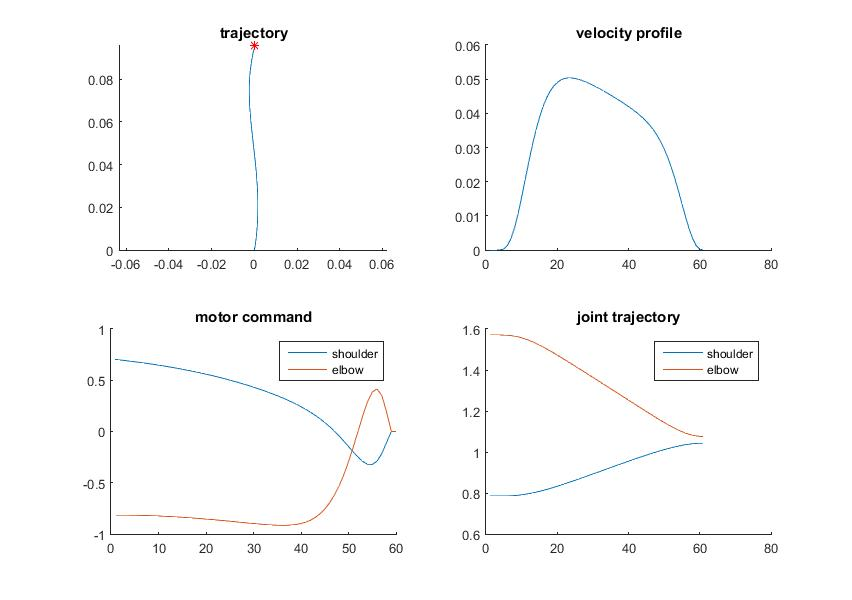
\includegraphics[width=\textwidth]{up8} 
	\caption{simulation result with high viscosity value}
	\label{fig:0.8}
\end{figure}
\begin{figure}[h]
	\centering
	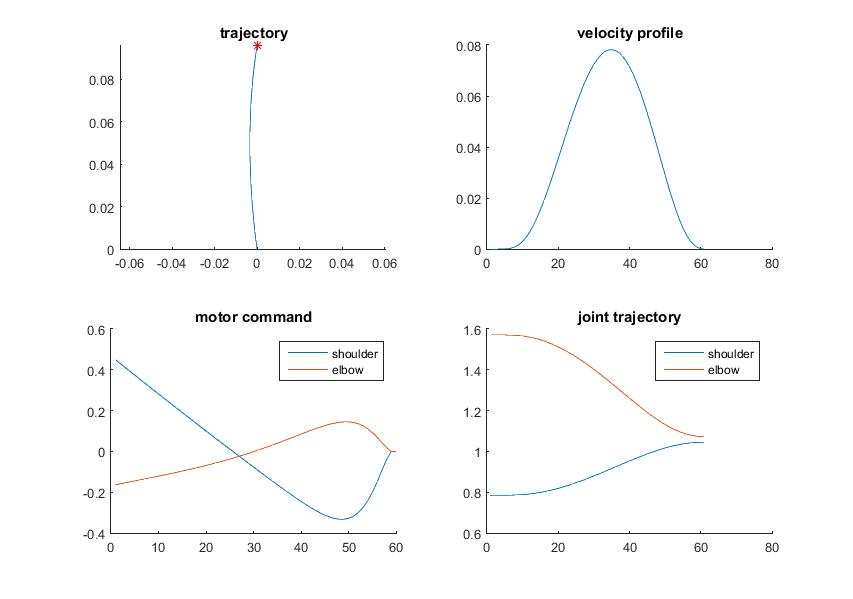
\includegraphics[width=\textwidth]{up0}
	\caption{simulation result with zero viscosity value}
	\label{fig 0.0}
\end{figure}